\documentclass[french,a4paper,DIV=11,numbers=noendperiod]{scrartcl}

% --- Encodage, langue, fontes ---
\usepackage{iftex}
\ifPDFTeX
  \usepackage[T1]{fontenc}
  \usepackage[utf8]{inputenc}
  \usepackage{lmodern}
  \usepackage[french]{babel}
\else
  \usepackage{fontspec}
  \usepackage{unicode-math}
  \defaultfontfeatures{Scale=MatchLowercase}
  \setmainfont{Latin Modern Roman}
  \setsansfont{Latin Modern Sans}
  \setmonofont{Latin Modern Mono}
  \usepackage[bidi=basic]{babel}
  \babelprovide[main,import]{french}
\fi

% --- Mise en page, microtypographie ---
\usepackage[margin=1.5cm]{geometry}
\usepackage{microtype}
\setlength{\parindent}{0pt}
\setlength{\parskip}{6pt}
\usepackage{ragged2e}
\usepackage[percent]{overpic} % coordonnées en %

% --- Maths ---
\usepackage{amsmath,amssymb}

% --- Sections non numérotées (style mémo/rapport court) ---
\setcounter{secnumdepth}{3}

% --- Couleurs, figures, tableaux ---
\usepackage{xcolor}
\usepackage{graphicx}
\usepackage{booktabs,longtable,tabularx,multirow}
\usepackage{float}
\usepackage{caption}
\usepackage{subcaption}

% --- Liens et URLs ---
\usepackage{xurl}
\usepackage{hyperref}
\usepackage[backend=biber,style=authoryear,maxcitenames=2,maxbibnames=99]{biblatex}
\addbibresource{references.bib}

% --- Compat Pandoc/Quarto ---
\providecommand{\tightlist}{\setlength{\itemsep}{0pt}\setlength{\parskip}{0pt}}

% --- Numéros de lignes (optionnel) ---
\usepackage[switch]{lineno}
\linenumbers
\modulolinenumbers[5]

% --- DEBUT ---

\title{Characterization and evolution of daily and hourly extreme precipitation in France using an Explicit-Convection Regional Climate Model}
\author{}
\date{}
\begin{document}
\maketitle


\textbf{Authors.}
Nicolas Decoopman, Juliette Blanchet (Univ. Grenoble Alpes, CNRS, INRAE,
IRD, Grenoble INP, IGE, 38000 Grenoble, France), Antoine Blanc (RTM,
ONF, 38000 Grenoble, France).

\textbf{Abstract.} Climate change is intensifying the global water cycle, with extreme precipitation events increasing in frequency and intensity at the global scale. While trends in daily precipitation extremes are well-documented, sub-daily extremes---critical for flash flood risk---remain poorly characterized, in particular in France, due to limited long-term, high-resolution stations. Convection-permitting models (CPMs) explicitly resolve deep convection and therefore offer the potential for a substantially improved representation of convective processes and short-duration precipitation extremes. This study evaluates the ability of the AROME regional climate model (2.5 km resolution, 1959--2022), forced by ERA5 reanalysis, to reproduce observed hourly precipitation extremes and their trends, using a dense network of Météo-France stations.

Using extreme value theory (GEV modeling), we analyze trends in
10-year return levels for both daily and hourly extremes. We show that at the daily
scale, AROME reproduces observed positive trends in southeastern France, consistent with
previous studies and Clausius--Clapeyron scaling. At the hourly scale,
trends are more heterogeneous and less robust, with high spatial variability
and low model-observation correlation.

Our results highlight the added value of explicit-convection models for
extreme precipitation studies, while underscoring their limitations for
convective extremes at resolutions coarser than 1 km. The Rhône Valley
emerges as a hotspot for intensifying hourly extremes. This work provides
the first national-scale assessment of hourly precipitation trends in
France, offering new insights for flood risk management and climate
adaptation strategies.

\textbf{Keywords.} Extreme precipitation, climate change,
convection-permitting model, AROME, sub-daily trends, France, extreme
value theory, flash floods, Clausius--Clapeyron scaling

\section{Introduction and context}\label{introduction-and-context}

\textbf{Climate change} is driving a warming of the planet's surface
air, with a more pronounced increase over land than over oceans  \parencite{IPCC2021}. Global warming has reached +1.1°C worldwide, +1.7°C in
metropolitan France, and +2°C in the French Alps compared to the
pre-industrial era. Furthermore, the Clausius-Clapeyron relationship
indicates that warmer air can hold more moisture (+7\% per °C)
\parencite{clapeyron1834}. Due to buoyancy (Archimedes' principle), warm air surrounded by cooler air tends to rise. As warm air ascends in the
atmosphere, it undergoes adiabatic cooling, leading to the condensation
of water vapor and the formation of precipitation \parencite{meteofrance}.
However, under calm conditions, the central portion of the precipitation
distribution does not fully capitalize on this excess moisture.
Energetic constraints (radiative balance, evaporation, ocean-air
exchanges) and dynamic constraints (subsidence, synoptic winds) limit
the increase in mean precipitation to only 1--3\% per °C \parencite{IPCC2021}. In
contrast, during intense convective events (thunderstorms, rapid
cyclogenesis), rapid ascent condenses nearly all of this surplus,
causing short-duration extreme rainfall to increase by 5--8\% per
°C---almost matching the theoretical potential. Extreme precipitation
closely follows the Clausius-Clapeyron scaling, whereas mean rainfall
remains influenced by numerous other energetic and dynamic factors
\parencite{ogorman2015contrasting}. Thus, climate warming theoretically leads to an
increase in extreme precipitation, though this increase varies with
changes in atmospheric circulation and can be locally amplified \parencite{blanchet2021explaining}.

\textbf{Extreme precipitation events} are defined as events belonging to the upper tail of the precipitation intensity distribution. There is no consensus
on what constitutes an extreme event. Some authors study
precipitation intensities above the 99th percentile or seasonal/annual
maxima, while others define extreme precipitation as events rarely or
never encountered in a human lifetime (e.g., precipitation levels
expected once every 10, 20, 50, 100 or 10 000 years). Extreme events are at the
heart of climate and societal concerns, as they account for the majority
of costs associated with flooding, landslides, and infrastructure
failures \parencite{IPCC_2022_WGIII}. In 2024, numerous such events made headlines,
including in Nepal, Afghanistan, Central Europe, eastern Spain, and
France \parencite{wmo2024}. Notably, in France in June
2024, intense high-altitude rainfall contributed to major flooding in
the Écrins massif \parencite{Blanc2024}; in October 2024, over 600 mm of
rain in 48 hours caused widespread flooding in the Ardèche department
\parencite{MeteoFrance2024_episodesArdeches}; and in May 2025, extremely intense but short-lived
thunderstorms (locally exceeding 120 mm/h) caused extensive damage in
southern Var \parencite{MeteoFrance2025}.

\textbf{Daily precipitation extremes} have increased in intensity and
frequency across more than half of the world's land regions, at a rate
close to +7\% per °C of warming \parencite{IPCC2021}. Some regional studies
suggest similar trends in a significant proportion of land areas \parencite{Donat2016}. In France, however, signals are far more
heterogeneous and less pronounced than for temperature, with strong
regional variations. In most regions, trends remain weak or
non-significant, and only in certain areas---particularly the
southeast---are clear signals detected. In this region, the frequency of
extreme Mediterranean episodes (cumulated rainfall \textgreater{} 200 mm
in 24 hours) has doubled between 1961 and 2020, although interannual
variability remains high \parencite{meteofrance2024}. The mean intensity of
daily extremes has increased by +22\% between 1961 and 2015 \parencite{Ribes2019}. At the national scale, no significant trend was detectable in
annual maxima of daily precipitation until the 1990s. Since then, some
studies report increases of +20\% to +40\%, though these estimates
remain sensitive to the period and analytical method \parencite{Donat2016}. In the southeastern Alps, the increase in 20-year return
level daily precipitation in autumn (1958--2017) could reach an order of
magnitude comparable to its mean value (\textasciitilde+100\%) \parencite{blanchet2021explaining}. Projections indicate that a +4°C
warming scenario could lead to an average increase of
\textasciitilde+15\% in daily extreme rainfall across France, and up to
+20\% in the northern half \parencite{Soubeyroux01022015}. There remains
strong spatial and interannual variability \parencite{IPCC2021}.

\textbf{Hourly extremes}, measured at 1-hour or shorter time steps, are
essential for characterizing intense convective phenomena (thunderstorm
downpours, stationary thunderstorms) often responsible for flash floods.
Due to the lack of long, spatially dense time series, there is no
systematic global analysis of sub-daily trends; available data are often
sparse, short, and non-significant. Nevertheless, several regional
studies detect an intensification of hourly extremes across nearly all
continents, though global confidence in an overall increase remains very
low \parencite{IPCC2021}. Increases in extreme rainfall have been observed in the
United States, China (summer), Australia (annually), South Africa
(summer), India, Malaysia, and Italy. Depending on the method and
region, studies highlight sensitivities ranging from +7\% to +13\% per
°C---up to twice the Clausius-Clapeyron rate \parencite{molnar2015relation}. In
France, few regional studies explicitly characterize this increase in
hourly extremes. Observed maximum 1-hour values now reach 40--60 mm
during major Mediterranean events, compared to 30--40 mm in the
1980s--1990s \parencite{meteofrance2024}. Only the study by \parencite{Berghald2025} appears to quantify trends in hourly extremes in the French Alps.
However, trends in hourly return levels remain weak to non-significant,
with no clear spatial or seasonal coherence, contrasting with the robust
signals observed at daily time scales \parencite{Soubeyroux01022015}. This suggests that hourly extremes do not yet show a clear climate signal, possibly because the signal is still emerging but cannot be robustly detected given the short length of available series and the high year-to-year variability.

\textbf{In France}, a nationwide network of daily precipitation with good spatial coverage became available from the 1950–1960s. At the hourly scale, most records date after the 1990–2000s. 

\textbf{In contrast, climate models} forced by reanalyses show the advantage of: 1) precipitation series that potentially go back further in time than raingauge records; and 2) spatially complete and
physically consistent fields, particularly useful in poorly instrumented
areas. Global Circulation Models (GCMs) are not suitable for studying convective extremes, as convection is parameterized, leading to over-smoothed and
poorly located hourly precipitation at resolutions of 12--200 km \parencite{KilometerScaleClimateModelsProspectsandChallenges}. The
emergence of regional climate models with explicit convection (CPMs,
Convection-Permitting Models) offers a unique opportunity: they
realistically simulate the dynamics of intense precipitation at fine
spatial and temporal scales over long periods. In France, the regional climate model with explicit convection CP-RCM AROME model (2.5 km) forced by ERA-Interim (80 km, 1979-2019) has been studied by \cite{Caillaud2021}, who show that CNRM-AROME realistically reproduces the location, intensity, frequency and interannual variability of northwestern Mediterranean heavy precipitation events at daily and especially hourly scales, with clear added value compared to the coarser CNRM-ALADIN RCM, albeit with some remaining regional biases in extremes. A new generation of simulation is now available, where CP-RCM AROME is forced by ERA5 (25-31km) from 1959 to 2022 This provides a unique dataset with sufficiently long series (63 years) to study precipitation extremes in France and their trends. However, the validity of the extremes simulated by this model has never been evaluated. Our study
addresses this gap by assessing the ability of the CP-RCM AROME model to reproduce observed hourly extremes, comparing modeled and observed
trends over several decades. It thus makes a dual contribution: 1)
methodological, by evaluating new simulations against extreme
stations; and 2) climatic, by documenting for the first time the
temporal evolution of hourly extremes in France over 60 years using a
validated explicit-convection model. This work sheds light on how hourly
extremes evolve in a warming climate while assessing the relevance of
CPMs for hydrometeorological impact studies at the local scale.

\section{Data used}\label{data-used}

\subsection{stations}\label{stations}

This work utilizes precipitation data from Météo-France stations
\parencite{meteofrance2024} at daily (1959--2022) and hourly (1990--2022) time
steps, as illustrated in Figure 1. At each spatial point, we calculate the proportion of missing data
in the time series for each season (or month) and year. We exclude years
where this proportion exceeds the 10\% threshold. The number of valid
remaining years is then derived. Only stations with at least
the minimum required number of years are retained (50 years for the
1959--2022 period and 25 years for the 1990--2022 period). Subsequent
analyses are restricted to this subset of stations and years.

\begin{center}
\includegraphics[width=\linewidth]{fig1.pdf}
\setcounter{figure}{0}% prochaine légende = Figure 1
\captionof{figure}{\small Distribution of the number of hydrological years with at most 10\% missing values for Météo-France stations at the daily (1959--2022) and hourly (1990--2022) time steps.}
\end{center}

Figure 1 highlights the strong contrast between daily and hourly observational records available in France. Daily stations (left) provide long, dense time series: more than half of the 8 198 stations have over 40 years of data with limited missing values, and several exceed 60 years. In contrast, hourly stations (right) remain much shorter: most of the 2 315 stations offer only 15–30 years of reliable data, reflecting the later deployment of automatic networks. This disparity underscores why long-term trends in sub-daily extremes are more difficult to detect than at the daily scale.

\subsection{AROME model}\label{arome-model}

The CP-RCM AROME model, recently forced by the ERA5 reanalysis, provides
hourly precipitation data from 1959 to 2022 at a 2.5 km resolution over
the computational domain shown in Figure 2 (Centre National de
Recherches Météorologiques 2014). This figure shows the spatial extent of the CP-RCM AROME computational domain, covering Western Europe and the northwestern Mediterranean region. In metropolitan France, 87,536 grid points are generated. 

\begin{center}
  \includegraphics[width=0.5\linewidth]{fig2.pdf}
  \captionsetup{type=figure}
  \setcounter{figure}{1}% la prochaine valeur utilisée sera 2
  \captionof{figure}{\small Mapping of the computational domain of the AROME numerical model.}
\end{center}

CP-RCM AROME model shows a generally good representation of heavy precipitation events, but several systematic biases are documented by \cite{Caillaud2021}. The model tends to underestimate the most intense daily and hourly extremes, particularly for the highest values (>200 mm/d and >40 mm/h). AROME also exhibits seasonal temperature biases: a cold bias in winter–spring, and a warm bias in summer associated with an excess of incoming short-wave radiation linked to underestimated cloud cover. In mountainous areas, the model is too cold and too wet, and snow cover tends to persist unrealistically above roughly 2000 m. Some precipitation-system properties (extent, duration, volume) also remain biased when compared with reference products. It should be note that temperature trends in the model are twice as weak as observed trends (personnal communication with CNRM researchers). It is therefore
important to note that the Clausius-Clapeyron-related component of
extreme trends will theoretically be half as strong as observed trends.

\section{Methodology}\label{methodology}

\subsection{Climatology}\label{climatology}

This study focuses on metropolitan France. The primary objective is to
validate the model (AROME grid points) against stations
(Météo-France stations) using simple yet representative precipitation
regime indicators (correlation and bias). This step is first conducted under
stationary conditions to focus on the climatology, then in a non-stationary context to assess trends and variability of extremes.

Seasons are defined as follows: \textbf{SON}: September (SEP), October
(OCT), November (NOV), \textbf{DJF}: December (DEC), January (JAN),
February (FEB), \textbf{MAM}: March (MAR), April (APR), May (MAY),
\textbf{JJA}: June (JUN), July (JUL), August (AUG) and \textbf{OND}:
October (OCT), November (NOV), December (DEC), \textbf{JFM}: , January
(JAN), February (FEB), March (MAR), \textbf{AMJ}: April (APR), May
(MAY), June (JUN), \textbf{JAS}: July (JUL), August (AUG), September
(SEP). The hydrological year (\textbf{YEAR}) is defined as the period
from 1 September of year N to 31 August of year N+1.

Using data from Météo-France stations and AROME simulations, the
following metrics were computed for each AROME grid point or station,
year, and month/season over the periods 1959--2022 and 1990--2022: rainy
days (threshold: $\geq$ 1 mm/day), average cumulative precipitation, average maximum of daily and hourly precipitation.

\subsection{Trends in extremes}\label{trends-in-extremes}

\subsubsection{GEV distribution for extremes}\label{gev-distribution-for-extremes}

While descriptive statistics provide useful summaries, they cannot: assess quality of very rare occurrence, e.g. of 10 year return events that are exceeded on average only once every 10 years. Furthermore, the descriptive statistics of Section 3.1 are stationary, thus they cannot inform about potential trends. To address
these limitations, we apply extreme value theory (EVT) \parencite{coles2001introduction}. This states that, under general conditions, the CDF of block maxima - e.g. annual maxima - can be approximated by the Generalized Extreme Value (GEV)
distribution.

At a the GEV distribution is a continuous
probability distribution parameterized by the triplet
\(\theta = (\mu, \sigma, \xi)\) --- respectively the location, scale
(strictly positive), and shape---with the following cumulative
distribution function: \[
F(x;\mu ,\sigma ,\xi) = \exp\left\{-\left[1 + \xi\frac{x - \mu}{\sigma}\right]^{-1/\xi}\right\}, \quad 1 + \xi\frac{x - \mu}{\sigma} > 0
\]

It unifies the three classical distributions Gumbel (\(\xi \to 0\)), Fréchet (\(\xi > 0\)) and Weibull (\(\xi < 0\)) where the shape parameter \(\xi\) determines the tail behavior.

\subsubsection{Non stationary GEV}\label{non-stationary-gev}

To consider trends in extremes, the GEV distribution can be made non-stationary
by allowing at least one GEV parameter to vary with time: $\mu(t)$, $\sigma(t)$
and/or $\xi(t)$. Owing to the difficulty of estimating the tail parameter $\xi$,
it is assumed stationary, i.e. $\xi(t) = \xi_0$. Three non-stationary models are
considered:

\[
\begin{array}{c@{\qquad}c@{\qquad}c}
% -------- Column 1 --------
\begin{array}{c}
\begin{aligned}
M_1(\theta_1)\\[-0.2ex]
\theta_1 = (\mu_0, \mu_1, \sigma_0, \xi_0)
\end{aligned}\\[0.4ex]
\begin{cases}
\mu(t) = \mu_0 + \mu_1\, t \\
\sigma(t) = \sigma_0 \\
\xi_0
\end{cases}
\end{array}
&
% -------- Column 2 --------
\begin{array}{c}
\begin{aligned}
M_2(\theta_2)\\[-0.2ex]
\theta_2 = (\mu_0, \sigma_0, \sigma_1, \xi_0)
\end{aligned}\\[0.4ex]
\begin{cases}
\mu(t) = \mu_0 \\
\sigma(t) = \sigma_0 + \sigma_1\, t \\
\xi_0
\end{cases}
\end{array}
&
% -------- Column 3 --------
\begin{array}{c}
\begin{aligned}
M_3(\theta_3)\\[-0.2ex]
\theta_3 = (\mu_0, \mu_1, \sigma_0, \sigma_1, \xi_0)
\end{aligned}\\[0.4ex]
\begin{cases}
\mu(t) = \mu_0 + \mu_1\, t \\
\sigma(t) = \sigma_0 + \sigma_1\, t \\
\xi_0
\end{cases}
\end{array}
\end{array}
\]


Furthermore, based on previous studies of trends in extremes in France
\parencite{Blanchet2018,Ribes2019}, we consider the case of a
trend starting at year $t_{+}=1985$, leading to the three models
$M_{1}^{*}$, $M_{2}^{*}$, and $M_{3}^{*}$. For example, in $M_{1}^{*}$:

\[
\mu(t)=
\begin{cases}
\mu_{0} & \text{if } t \le 1985,\\[4pt]
\mu_{0} + \mu_{1}(t-1985) & \text{if } t \ge 1985.
\end{cases}
\]

This gives six non-stationary models, in addition to the stationary model denoted ($M_0$), which corresponds to $\mu(t)=\mu_0$, $\sigma(t)=\sigma_0$, and $\xi(t)=\xi_0$.

\subsubsection{Return level}\label{return-level}

The return level (or quantile of order \(1 - \tfrac{1}{T}\)) in a GEV
distribution corresponds to the threshold value exceeded, on
average, once every \(T\) years. For a non-stationary GEV with parameters $\mu(t)$, $\sigma(t)$ and $\xi_{0}$,
the distribution is a function of the year $t$.
Denoting by $F^{-1}_{t}$ the quantile function of the non-stationary GEV, it is given by:

\[
\begin{equation}\label{eq:RL}
\mathrm{RL}_{T}(t)
= F^{-1}_{t}\!\left(1 - \frac{1}{T}\right)
=
\begin{cases}
\mu(t) + \dfrac{\sigma(t)}{\xi_{0}}
\left[
\left( -\log\!\left(1 - \dfrac{1}{T}\right) \right)^{-\xi_{0}}
- 1
\right]
& \text{if } \xi_{0} \ne 0, \\[10pt]
\mu(t) - \sigma(t)\,
\log\!\left( -\log\!\left(1 - \dfrac{1}{T} \right) \right)
& \text{if } \xi_{0} = 0 \quad \text{(Gumbel)}.
\end{cases}
\end{equation}
\]

Owing to the linear form of $\mu(t)$ and $\sigma(t)$ in the considered
non-stationary models, return levels are linear functions of time in
models $M_{1}$, $M_{2}$, and $M_{3}$, and linear only after 1985 in the
breakpoint models $M_{1}^{*}$, $M_{2}^{*}$, and $M_{3}^{*}$. In the
stationary model $M_{0}$, return levels are of course constant over time.
For the non-stationary models, the relative trend in the $T$-year return
level (\%) between 1985 and 2022 is computed as

\[
\mathrm{Trend} =
\frac{\mathrm{RL}_{T}(2022)-\mathrm{RL}_{T}(1985)}
{\mathrm{RL}_{T}(1985)}.
\]

\subsubsection{Maximum likelihod estimation and confidence intervals for the return levels}\label{maximu-likelihood-estimation-and-confidence-intervales}

The GEV parameters $\theta$ are estimated by maximum likelihood method for each
spatial location separately, considering the block maxima at a given
location to be independent. This gives a set of parameters $\hat{\theta}$,
i.e.\ the estimators $\hat{\mu}(t)$, $\hat{\sigma}(t)$, $\hat{\xi}_{0}$ and thus
return level estimates $\widehat{\mathrm{RL}}_{T}(t)$ from Eq.~1. Noting that the
$T$-year return level function can be written as
$\mathrm{RL}_{T}(t)=\mathrm{RL}_{T,0}+\mathrm{RL}_{T,1}\, t$
for models $M_{1}$, $M_{2}$, $M_{3}$ and
\[
\mathrm{RL}_{T}(t)=
\begin{cases}
\mathrm{RL}_{T,0} & \text{if } t<1985,\\[4pt]
\mathrm{RL}_{T,0}+\mathrm{RL}_{T,1}(t-1985) & \text{if } t>1985,
\end{cases}
\]
for models $M_{1}^{*}$, $M_{2}^{*}$, $M_{3}^{*}$,
confidence intervals for the trend coefficient $\mathrm{RL}_{T,1}$ are obtained
by profiling the likelihood with respect to $\mathrm{RL}_{T,1}$ \parencite{coles2001introduction}. If
the $90\%$ confidence interval of $\mathrm{RL}_{T,1}$ does not contain $0$, the
$T$-year return level trend is not significant at level $10\%$.

\subsubsection{Model selection}\label{model-selection}

At each spatial point, we consider the models
\(M_0, M_1, M_2, M_3, M_1^\ast, M_2^\ast\), and \(M_3^\ast\) that we temporarily rename $M_{0}$ to $M_{6}$. Let
\(k_j\) denote the number of parameters in model $M_{j}$ for $j = 0,\dots,6$. We apply for each non-stationary model $M_{j}$, $j \ge 1$, a likelihood ratio test to compare the goodness of fit of $M_{j}$ to that of the stationary model $M_{0}$, accounting for their number of parameters to avoid overfitting. Let $p_{j}$ be the corresponding $p$-value. 

\[
\Lambda_{j}=2\bigl(\ell_{j}-\ell_{0}\bigr) \overset{H_0}{\sim}\chi^{2}_{\;k_j-k_0} \quad \text{with} \quad p_{j}= \mathbb{P}(\chi^{2}_{k_j-k_0}\ge \Lambda_{j}\bigr)
\]

If $p_{j} \le 10\%$, the model $M_{j}$ is considered to perform better than $M_{0}$, otherwise $M_{0}$ is selected. If several models $M_{j}$ are preferred to $M_{0}$, we apply the following procedure: 1) if either $M_{3}$ or $M_{3}^{*}$ are preferred to $M_{0}$, we select among these two models that with the smallest $p$-value among $p_{3}$ and $p_{3}^{*}$; 2) otherwise, we select among $M_{1}$, $M_{1}^{*}$, $M_{2}$, $M_{2}^{*}$ that with the smallest $p$-value among $p_{1}$, $p_{1}^{*}$, $p_{2}$, $p_{2}^{*}$.

This two-step process prioritizes models with simultaneous temporal
effects on \(\mu\) and \(\sigma\) when statistically justified, ensuring
complexity is introduced only when it provides credible information. In the rest of the article, only the selected model is considered at each location (grid point or station).

\subsection{Assessing the agreement between AROME and the stations}\label{assessing}

The stations and CP-RCM AROME for the descriptive statistics of Section 2 and the trends in the 10-year return level derived from the best model (see Section 3.2.5). We evaluate the agreement between each
Météo-France station is matched to the corresponding AROME grid point
(2.5 km × 2.5 km) based on its spatial location. This
correspondence allows calculating the Pearson correlation (\(r\)) and
mean error (\(ME\)) between observed and simulated statistics.

\section{Results}\label{results}

We begin by evaluating, grid point by grid point, the ability of AROME
to reproduce the precipitation regime observed by Météo-France stations.
This initial stationary evaluation allows asessing the quality of the climatology before examining the return level trends.

\subsection{Evaluation of the precipitation climatology of
AROME}\label{evaluation-of-the-precipitation-climatology-by-arome}

\subsubsection{Spatial representation}

Over the period 1959--2022 (Figure 3, first column), AROME slightly
overestimates the \textbf{annual frequency of precipitation days}: +6.35
days/year (i.e., +5.56\%). However, significant local biases persist:
over +30 days for several stations in the Massif Central and the
Pyrenees, while negative biases (−10 to −30 days) are concentrated in
the Northern Alps, Brittany, and Alsace. The spatial correlation is
high (\emph{r} = 0.95), indicating that the model correctly reproduces
the major regional patterns. AROME and stations agree on locating
maximum frequencies over mountainous regions (Alps, Pyrenees, Massif
Central, Vosges, Jura), with more than 140--160 days/year, and also high
values over the Atlantic Grand Ouest (Brittany, Normandy, Pays de la
Loire: 80--120 days/year). Conversely, the Mediterranean coast and the
Provence region remain the driest in terms of frequency, often
\textless{} 50--70 days/year.

Over the period 1959--2022 (Figure 3, second column), AROME accurately
estimates the \textbf{annual cumulative precipitation}: +11.48 mm/year
(i.e., +1.23\%). However, significant local biases persist: over +300
mm/year for all stations along the Pyrenean ridge and the Chamonix
station, while negative biases (−100 to −400 mm/year) are concentrated in
the Northern Alps, the Basque Coast, and Alsace. The spatial correlation
is high (\emph{r} = 0.94), indicating that the model correctly
reproduces the major regional gradients. The southwestern Atlantic coast
(Pyrenees, Aquitaine) and the Northern Alps receive the highest
cumulative precipitation (over 1800 mm/year). The Massif Central and inland reliefs (Vosges, Jura) show intermediate cumulative values (900--1460 mm/day). The Mediterranean coast (Languedoc, Provence) remains generally
drier (\textless{} 550 mm/day), despite occasional intense rainfall.
These results are consistent with hourly data from 1990 to 2022
(Appendix 2-2.3).

Over the period 1959--2022 (Figure 3, third column), AROME slightly
underestimates the \textbf{average of daily maximum precipitation}:
-1.18 mm/day (i.e., -2.35\%). Significant local biases remain: deficits
of −5 to less than −20 mm/day across the Cévennes, extending to the
northern edge of the Northern Alps, the southeastern coast, and the
Basque Coast; up to −5 mm/day over a large part of central France and
Alsace; and +5 to +20 mm/day over the Pyrenean ridge, the western
foothills of the Cévennes, and the Northern Alps. The spatial
correlation is high (\emph{r} = 0.96), indicating that the model
correctly reproduces the major regional gradients. The highest average
daily precipitation maxima occur in the Cévennes and, more generally, on
the southeastern side of the Massif Central (approximately 100--125
mm/day). Alpine and Pyrenean reliefs also show high maxima (80--100
mm/day). The Atlantic coast and the Paris Basin exhibit more moderate
maxima (30--60 mm/day), while Provence and the Côte d'Azur, despite
lower frequency, can locally experience very heavy storms (40--80 mm/day
on average).

Finally, at hourly time steps (Figure 3,
fourth column). Over the period 1990--2022, AROME significantly
underestimates the \textbf{average of hourly maximum precipitation}:
-3.42 mm/h (i.e., -18.65\%). Significant biases persist: deficits of −5
to less than −10 mm/h over almost all of France, particularly in the
Cévennes and the Rhône Valley. The spatial correlation remains high
(\emph{r} = 0.89), confirming a good representation of the spatial variability already observed at the daily scale. Regarding seasons, the
bias ranges from −0.02 mm/h (DJF) to −3.75 mm/h (JJA), suggesting a
marked underrepresentation of summer convective extremes.

\begin{figure}[htbp]
    \centering
    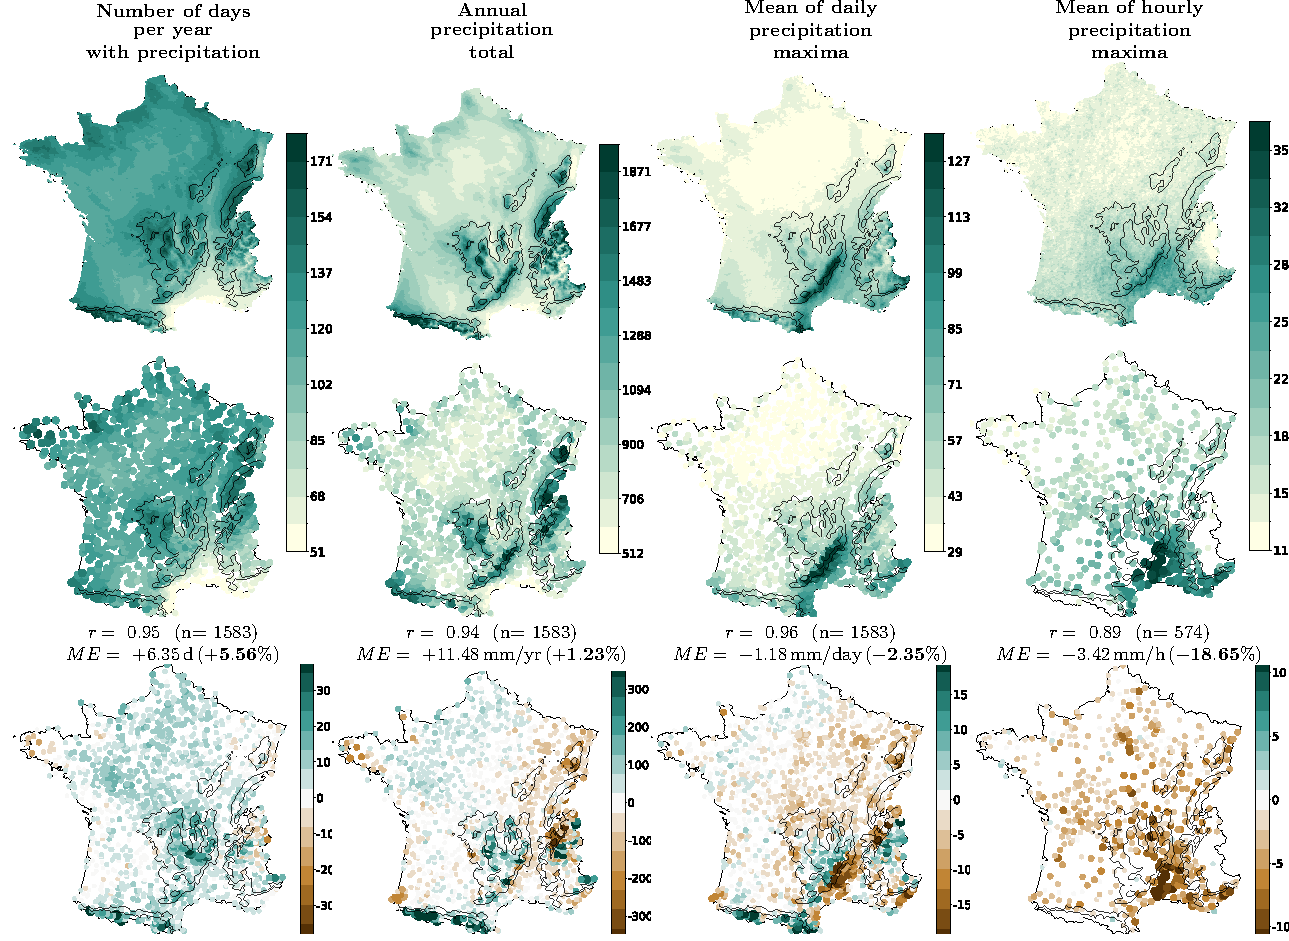
\includegraphics[width=\textwidth]{fig3.pdf}
    \setcounter{figure}{2}% prochaine légende = Figure 3
    \caption{\small Climatology between the AROME model (first row), Météo-France stations (second row) with the correlation ($r$) and the number of stations compared (n), and the AROME–Station difference (third row) with the bias ($ME$) and the associated relative deviation (\%) derived from daily data from 1959 to 2022 and hourly data from 1990 to 2022 for a hydrological year. The contour lines show the 400 and 800 m isolines. To ease visualization, colour scales are symmetrically saturated. Depending on the statistic, we apply a saturation threshold (99.9\% for the number of days and 99\% for annual and mean of maxima precipitation). All maps are clipped to this common percentile range.}
\end{figure}

\subsubsection{Correlations of climatological data}

Regardless of the indicator (Figure 4), the AROME model faithfully
reproduces stations, with a minimum correlation of 0.64.
Irrespective of the temporal scale---daily (1959--2022 or 1990--2022) or
hourly (1990--2022)---and the season, the simulated fields agree very
well with the raingauge data: correlation ranges from 0.92 to 0.98 for the
number of rainy days and cumulative precipitation. This performance is
maintained for the mean of daily maxima (periods 1959--2022 and
1990--2022) over the hydrological year, autumn, winter, and spring, but
degrades in summer (\textbf{JJA}), with a correlation of 0.85. At the
hourly scale, the quality of the mean maxima further
deteriorates: correlation drops by up to 0.3 points, falling to 0.70 in
spring (\textbf{MAM}) and summer (\textbf{JJA}), and to 0.64 in spring
(\textbf{AMJ}). AROME under-represents summer convective extremes,
especially at the hourly scale, despite a well-captured spatial
structure. In April, the bias is +0.22 mm/h (i.e., +3.76\%); in May,
-0.20 mm/h (i.e., -2.42\%) over half of France; and in June, -1.68 mm/h
(i.e., -18.29\%) across all of France. The spatial correlation remains high
in April (\emph{r} = 0.83). \emph{r} = 0.60 in May and 0.63 in June.

\begin{figure}[htp]
\centering
    \includegraphics[width=0.85\textwidth]{fig4.pdf}
    \captionsetup{type=figure}
    \setcounter{figure}{3}% prochaine légende = Figure 4
    \caption{\small Correlations of climatological data between the AROME model and Météo-France stations for each data source.}
\end{figure}

\subsection{Evaluation of extreme precipitation
trends}\label{evaluation-of-extreme-precipitation-trends}

\subsubsection{Daily}

Starting with the \textbf{daily scale}, Figure 5 shows quite complicated patterns of trends in 10-year return levels for the hydrological year as for the seasons. Despite this complexity, similar patterns of trends are notably found for AROME and for the stations, with however a tendency of AROME to show weaker trends. Over the hydrological year (\textbf{YEAR}), only the Mercantour region stands out with
a significant increase of between +20\% and +30\%. The stations also show a
generalized positive signal along the Rhône Valley, with trends ranging
from +5\% to \textgreater+30\%. Outside these areas, trends are weak, of
variable sign, and most often not significant, which argues for a
seasonal analysis. In autumn (\textbf{OND}), AROME indicates negative
trends (−10\% to \textless−30\%) over the Paris Basin, the western slope
of the Massif Central, and the Prealps, and a marked increase in the
Mercantour, as previously observed. The stations confirm this pattern, but
with a less pronounced decrease in the Prealps and a clearer signal in
the Alps. The Rhône Valley stands out with increases locally reaching
+40\%. In winter (\textbf{JFM}), AROME highlights marked negative
trends---up to −40\%---in the Verdon and Haut-Var regions; more moderate
decreases (−15\%) also affect the Dordogne Valley, Limousin, and the
northern Massif Central. Conversely, the northern tip of France, the
Jura, and the Vosges show positive trends of +10\% to +30\%. The stations
confirm this pattern, while extending the area of decrease to the
Southern Alps and the French Riviera. In spring (\textbf{AMJ}), the
trends are less structured: AROME does not isolate any clear pattern
except for the Camargue coast (\textgreater+30\%). The stations show a
generalized increase over much of France, locally \textgreater+35\%. In
summer (\textbf{JAS}), AROME reveals a generalized decrease across
France, particularly in the southern half, reaching \textless−40\% in
the Pyrénées-Orientales. The stations confirm this spatial pattern,
accentuating it on the French Riviera. Overall, AROME reproduces the
spatial distribution of observed trends, but with low correlation and
sometimes reduced extent, with a mean bias ranging from -0.30\%
(\textbf{JFM}) to -5.44\% (\textbf{AMJ}).

\begin{figure}[htbp]
  \centering
  \nolinenumbers
  \setcounter{figure}{5}
  \begin{overpic}[width=\linewidth]{fig5.pdf}
    % Ajuster 73,6 (x,y en %) et la largeur 0.25\linewidth
    \put(55,12){%
      \colorbox{white}{%
        \parbox{0.40\linewidth}{\justifying\footnotesize
          {\figurename~\thefigure} — Relative trends from 1995 to 2022 (\%) in the 10-year return level of daily precipitation for AROME (left) and Météo-France stations (right), with the correlation ($r$), the number of stations compared (n), and the bias ($ME$). These results are derived by fitting, at each location, the selected GEV model to daily precipitation maxima from 1959 to 2022. The contour lines show the 400 and 800 m isolines. To ease visualization, colour scales are symmetrically saturated using a 99\% threshold. All maps are clipped to this common percentile range.%
        }%
      }%
    }
  \end{overpic}
  % évite une seconde légende visible mais garde la cohérence des flottants
  \captionsetup{labelformat=empty}
  \caption{}%
\end{figure}
\linenumbers

\subsubsection{Hourly}

Switching to the \textbf{hourly scale}, Figure 6 reveals spatial patterns that are markedly more heterogeneous and much less robust than those observed at the daily scale (Figure 5). The amplitude of trends is also much larger: the colour scale spans from $-100\%$ to $+100\%$, compared with roughly $-30\%$ to $+30\%$ in Figure 5. This difference in scale enhances visual contrasts and shows that hourly return levels fluctuate much more strongly from one location to another.

Over the hydrological year (\textbf{YEAR}), AROME shows weak and spatially inconsistent trends, with scattered decreases and isolated positive signals in the northern half of France and the Alps. The stations display an even stronger variability, with changes frequently reaching $\pm 50\%$ and sometimes exceeding $+100\%$. Correlations remain low ($r = 0.12$), and the mean bias ($ME = 29\%$) is higher than at the daily scale. In autumn (\textbf{OND}), AROME exhibits a mix of positive and negative trends without any clear spatial structure, while the stations show a strongly positive pattern (up to $+100\%$) along the French Riviera. In winter (\textbf{JFM}), AROME suggests weak decreases in the western and southern regions, whereas the stations record very pronounced and scattered increases (western France, eastern Pyrenees, Rhône Valley), ranging from $+80\%$ to $+100\%$. The near-zero correlation ($r = 0.02$) highlights the noisy nature of hourly signals. In spring (\textbf{AMJ}), the contrast in scale becomes even more evident: AROME shows only sparse and modest signals, whereas many stations display strong increases (often $> +60\%$ and locally approaching $+100\%$) across most of France. This leads to the highest mean bias ($ME = 60\%$). In summer (\textbf{JAS}), AROME indicates predominantly negative trends, rarely exceeding $-40\%$. The stations, however, show extremely high variability, commonly between $-100\%$ and $+100\%$, particularly in the Rhône Valley. This results in a very low correlation ($r = 0.04$) and a substantial bias ($ME = 19\%$).

Overall, Figure 6 shows that hourly extremes are far more volatile and less spatially coherent than daily extremes. The expanded $\pm 100\%$ scale highlights strong local fluctuations and explains the weak agreement between modelled and observed trends. Whereas AROME reproduced the main spatial patterns at the daily scale, it struggles to capture the fine-scale, high-frequency variability characteristic of hourly precipitation maxima.


\begin{figure}[htbp]
  \centering
  \nolinenumbers
  \setcounter{figure}{6}
  \begin{overpic}[width=\linewidth]{fig6.pdf}
    % Ajuster 73,6 (x,y en %) et la largeur 0.25\linewidth
    \put(55,12){%
      \colorbox{white}{%
        \parbox{0.40\linewidth}{\justifying\footnotesize
          {\figurename~\thefigure} — Relative trends from 1995 to 2022 (\%) in the 10-year return level of hourly precipitation for AROME (left) and Météo-France stations (right), with the correlation ($r$), the number of stations compared (n), and the bias ($ME$). These results are derived by fitting, at each location, the selected GEV model to hourly precipitation maxima from 1990 to 2022. The contour lines show the 400 and 800 m isolines. To ease visualization, colour scales are symmetrically saturated using a 90\% threshold. All maps are clipped to this common percentile range.%
        }%
      }%
    }
  \end{overpic}
  % évite une seconde légende visible mais garde la cohérence des flottants
  \captionsetup{labelformat=empty}
  \caption{}%
\end{figure}
\linenumbers

Given the persistent spatial heterogeneity of the seasonal trends (Figure 6), we refine the analysis at the monthly scale (Figure 7).
AROME indicates positive trends (+25\% to \textgreater+150\%) in the
Rhône Valley and the Prealps in February (\textbf{FEB}), over the
western Mediterranean arc (Roussillon--Lower Languedoc) in March
(\textbf{MAR}), and the eastern arc (Azur Basin) in November
(\textbf{NOV}). The stations confirm this pattern, markedly
strengthening the signal in the Rhône Valley in February, with trends
approximately twice as high as those estimated by AROME. In June
(\textbf{JUN}), both AROME and the stations show a predominantly
increasing signal across the entire territory, with local trends
sometimes exceeding +150\%. However, the extremely low spatial
correlation between the two datasets (\emph{r} = 0.10) indicates that,
while they usually agree in sign, the localization of trends is
inconsistent/noisy. This discrepancy, combined with high summer
convective variability and the short length of monthly series
(1990--2022), calls for caution.

\begin{figure}[htp]
\centering
    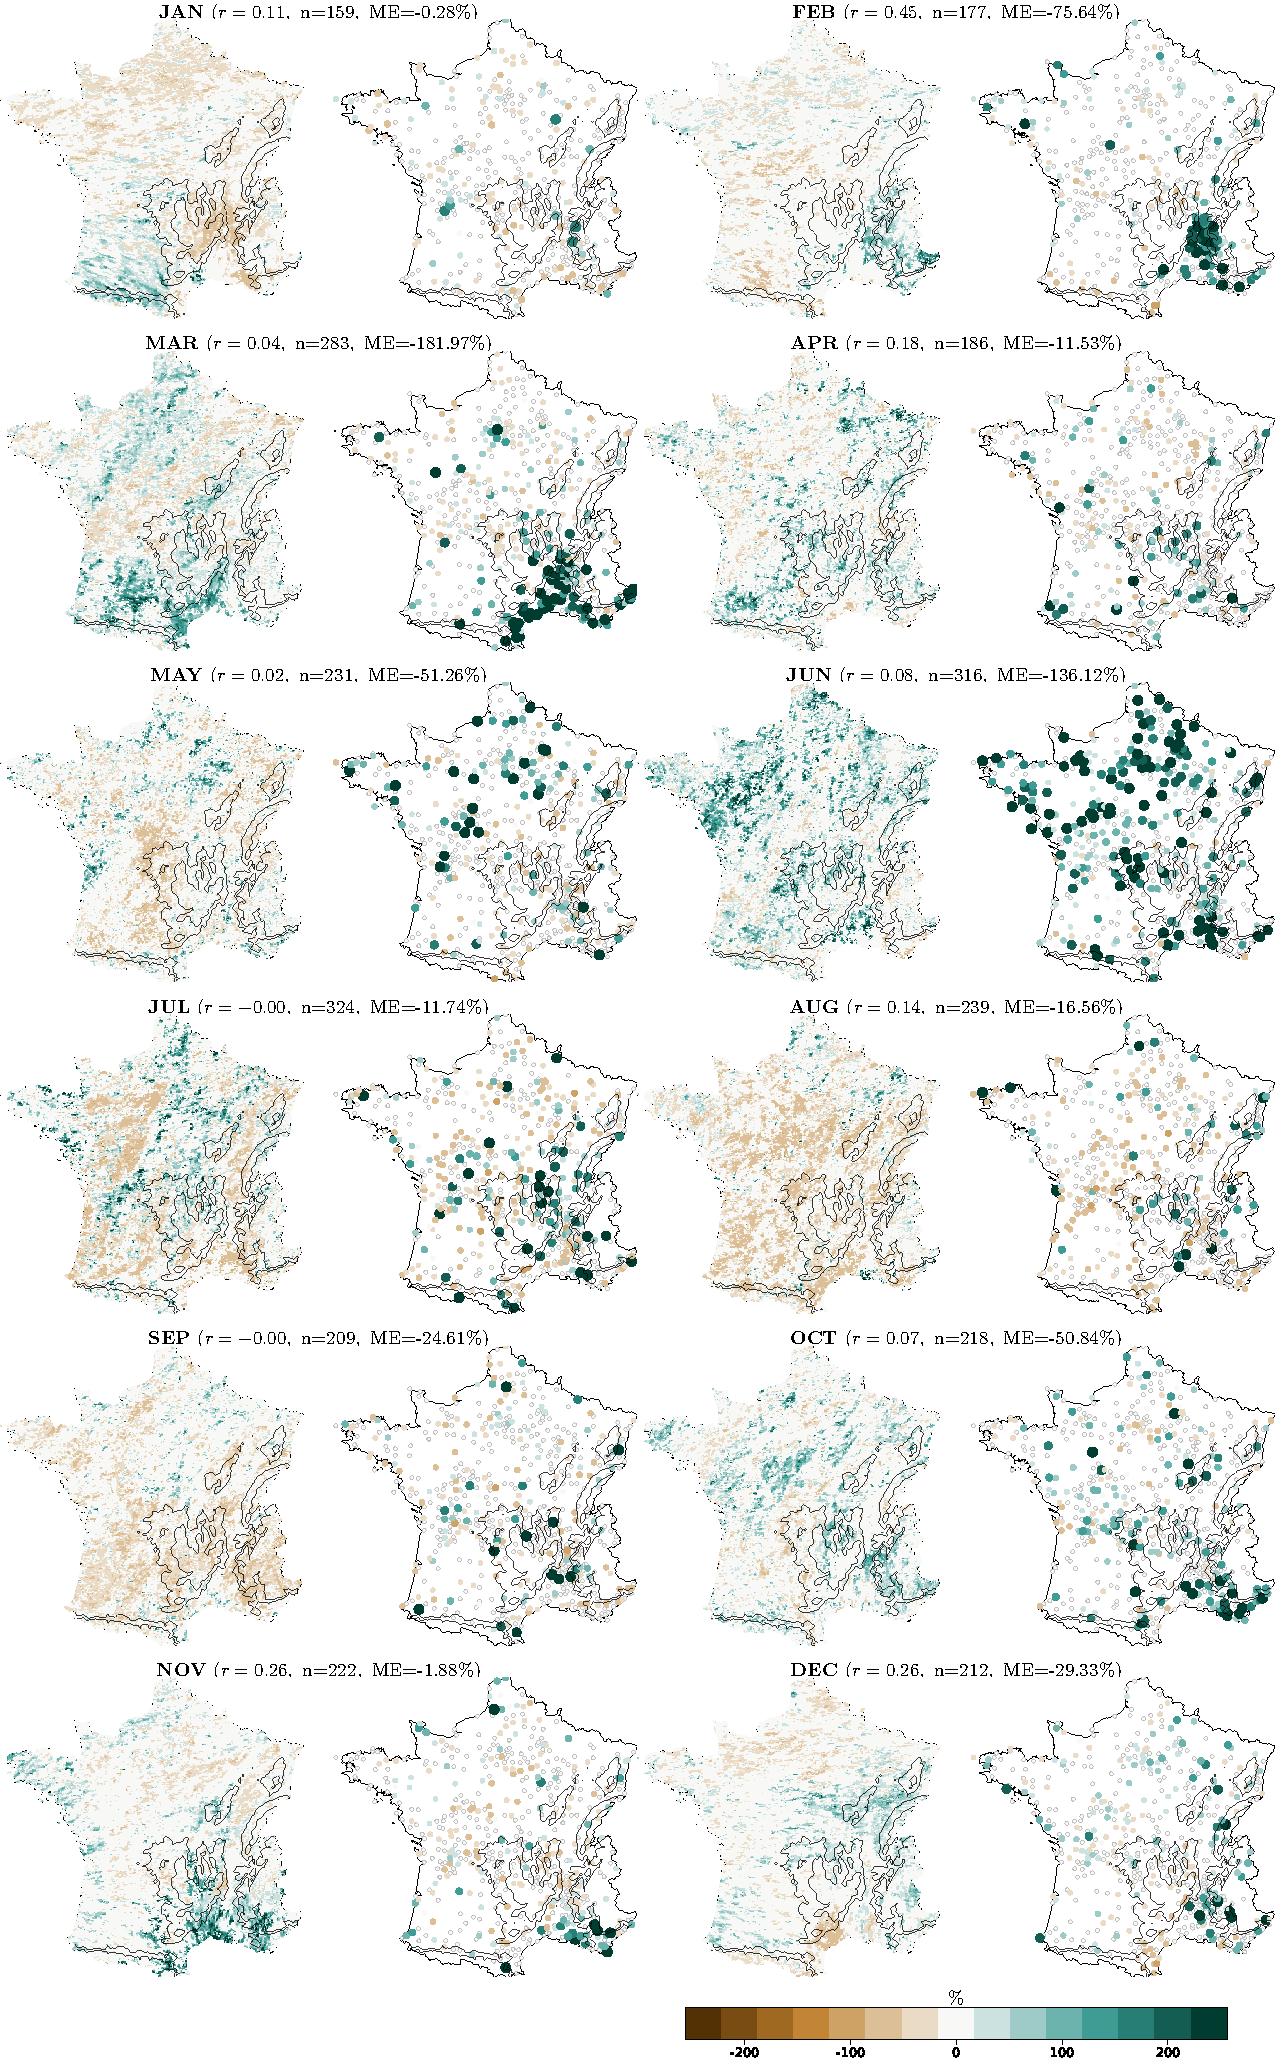
\includegraphics[width=\textwidth]{fig7.pdf}
    \captionsetup{type=figure}
    \setcounter{figure}{6}% prochaine légende = Figure 7
    \captionof{figure}{
        Relative trends from 1995 to 2022 (\%) in the 10-year return level of hourly precipitation for AROME (left) and Météo-France stations (right), with the correlation ($r$), the number of stations compared (n), and the bias ($ME$). These results are derived by fitting, at each location, the selected GEV model to daily precipitation maxima from 1959 to 2022. The contour lines show the 400 and 800 m isolines. To ease visualization, colour scales are symmetrically saturated using a 90\% threshold. All maps are clipped to this common percentile range.
        }
\end{figure}

\subsubsection{Spatial correlations}

To objectify these divergences, we now examine the spatial correlations between AROME and the stations,
by month, in order to identify where agreement is structural
and where it is mostly noise. At the daily scale (1959--2022), trend
correlations range from 0.10 (\textbf{JUN}) to 0.51 (\textbf{DEC}),
with several months reaching or exceeding 0.40 (\textbf{JAN},
\textbf{MAR}, \textbf{AUG}, \textbf{NOV}) (Figure 8). At the hourly scale
(1990--2022), seasons exhibit weak correlations ranging from 0.00
(\textbf{JAS}) to 0.09 (\textbf{OND}), and monthly correlations extend
from 0.02 (\textbf{SEP}, \textbf{OCT}) to 0.42 (\textbf{FEB}).

When restricting to trends significant by profile likelihood, the daily
scale (1959--2022) shows monthly values from 0.17 (\textbf{JUN}) to
0.77 (\textbf{DEC}), with other months also showing high correlation
(\textbf{JAN} 0.70; \textbf{MAR} 0.71; \textbf{NOV} 0.68; \textbf{AUG}
0.52). At the hourly scale (1990--2022), seasonal values cover −0.11--0.15 and monthly values −0.01--0.66.
Restricting to significant trends strongly increases daily correlations,
with high monthly maxima. The gain is pronounced in winter and late
summer/autumn (\textbf{JAN}, \textbf{MAR}, \textbf{NOV}, \textbf{DEC},
\textbf{AUG}). At the hourly scale, even after filtering, improvement
remains partial: some months improve (\textbf{FEB}), but several periods
are characterized by correlations near zero or slightly negative
(\textbf{MAY}, \textbf{SEP}).

\begin{figure}[htp]
\centering
    \includegraphics[width=\textwidth]{fig8.pdf}
    \captionsetup{type=figure}
    \setcounter{figure}{7}% prochaine légende = Figure 7
    \caption{\small Correlations of relative trends (all and significant) between AROME and Météo-France stations, by month.
Values above each bar indicate the number of stations used in the calculation.}
\end{figure}

\section{Discussion}\label{discussion}

\subsection{Climatology: consistencies, divergence and limitations}\label{climatology-consistencies-divergence-and-limitations}

The results confirm that AROME correctly reproduces the main rainfall
regimes over metropolitan France, as supported by the literature
\parencites{Fumiere2020,Caillaud2021,hess-28-2579-2024,LucasPicher2024}. It is able to reproduce the climatological orographic intensification of precipitation over the Alps,
the Pyrenees, and the Massif Central, a pronounced transition from Atlantic to continental climatic influence in the west, and the dryness of the Mediterranean
basin. This consistency with the stations indicates a satisfactory
representation of the dynamic forcings (moisture transport by westerly
flows, orographic uplift, low-level circulation in the Mediterranean).

AROME's ability to reproduce the frequency and quantity of precipitation
is maintained throughout the year, but performance declines for the
average of daily maxima in summer and even more so at the hourly scale.
The model underestimates high-intensity precipitation (\textgreater{} 40
mm/h \parencite{Caillaud2021,poncet2024convection}). Summer
convection remains partially under-resolved despite the 2.5 km spatial
resolution. In this study, we showed (results not shown) that
correlation increases (+30\%) when the time window is extended to 6 or 9 hours.
For such events, AROME may still simulate the same thunderstorm cell but with timing errors (starting too early or too late), by spreading its intensity over several nearby grid points—which cannot be fully evaluated given the sparse station network—and by underestimating the local peak precipitation. The 2--3
km grid spacing is a major step forward for representing convection
without parameterization, but it remains too coarse for applications
sensitive to intense maxima \parencite{prein2015regional}. Our evaluation compares point-scale raingauge measurements with 2.5 km × 2.5 km AROME grid-box averages. This mismatch in spatial support is relatively modest for daily accumulations, but it becomes a major limitation at the hourly scale: a single convective core may affect only part of a grid cell, so that local station extremes can be much higher (or lower) than the corresponding AROME value even when the event is realistically simulated at the grid-box scale. A high-resolution gridded observational product would therefore be better suited to evaluating hourly extremes than individual stations. In this respect, Météo-France’s COMEPHORE product – a 1 km, hourly radar–gauge precipitation reanalysis over metropolitan France – would be particularly valuable \parencite{MeteoFrance_COMEPHORE_dataGouv}. It would have been interesting to include COMEPHORE in this study, but the reanalyses only begin in 1997, with poor quality over the Alps before 2007 \parencite{Fumiere2020}.

\subsection{Trends in precipitation extremes: consistencies,
divergences, and
limitations}\label{trends-in-precipitation-extremes-consistencies-divergences-and-limitations}

\subsubsection{Daily data}

The positive and significant daily trends identified from the
\emph{stations} over several regions of France are consistent with the
IPCC assessment that heavy precipitation and associated extremes have
increased in intensity and frequency over many land regions, especially
in mid-latitudes \parencite{IPCC2021}. The stations highlight clear
hotspots in the Rhône Valley and the southern Alps (+5 to +30%), in
agreement with regional studies documenting an intensification of daily
extremes in southeastern France
\parencite{Blanchet2018,blanchet2021explaining,Ribes2019}. In northern
France, the marked increases (locally up to +35%) are broadly
consistent with national projections indicating stronger increases in
daily extremes in the northern half of the country under a +4 °C warming
scenario \parencite{soubeyroux:hal-04991790}. In southeastern France,
however, the spatial patterns differ from these projections, partly
because Soubeyroux et al. analyse 100-year return levels while we focus
on 10-year return levels, and partly due to methodological and model
differences.

The \emph{AROME} simulation reproduces the same large-scale spatial
organisation of daily trends as the stations but with weaker amplitudes.
This attenuation is consistent with the known underestimation of extreme
precipitation in AROME and with the spatial smoothing inherent to
grid-box values.

\subsubsection{Hourly data}

At the hourly scale, the \emph{stations} exhibit weaker and often
non-significant spatial trends, consistent with the IPCC’s assessment of
low confidence in global sub-daily extreme precipitation trends due to
short, sparse, and heterogeneous records \parencite{IPCC2021}. Despite
this, the stations show coherent increases in several months:
February (Rhône Valley, Pre-Alps), March (western Mediterranean arc),
and November (eastern Mediterranean arc). In June, stations display a
widespread increase (up to +150%), reflecting the dominance of highly
localised convective events. A sensitivity analysis (not shown) confirms
that these increases do not result from a single anomalous year but from
a succession of intense events during the last decade.

The \emph{AROME} simulation broadly reproduces the monthly structure of
the signals but with substantially weaker amplitudes (e.g. February in
the Rhône Valley, where AROME trends are roughly half of those observed
at stations). The limited period (1990–2022) reduces statistical power,
and interannual convective variability can mask or mimic trends. In
June, the very low spatial agreement between AROME and the stations
illustrates a representativeness mismatch: isolated convective cells may
affect a station without influencing the full 2.5 km grid box, or
vice-versa. This mismatch becomes the dominant source of discrepancy,
highlighting the limited relevance of monthly diagnostics for extremes.

Regional studies report sensitivities of +7 to +13\%/C for sub-daily
extremes—sometimes exceeding Clausius–Clapeyron scaling for short-lived
convective events \parencite{molnar2015relation}. In contrast, AROME
shows almost no clear signal in hourly return levels and strongly
underestimates trends, which is expected given that temperature trends
in AROME are about half the observed warming, implying that CC-related
precipitation sensitivities should also be reduced in the model.

\subsection{Statistical robustness of
the trends with respect to the considered period}\label{statistical-robustness}

Considering a long window (1959--2022) allows reducing estimation uncertainties and sampling
several climate regimes (global dimming phase dominated by aerosols
until the 1980s, then accelerated warming from the late 1980s--1990s).
Conversely, 
a short window (1990--2022) isolates the regime dominated by a rapid
warming, the decrease in sulfate aerosols in Europe, and the
quasi-linear increase in water vapor content (+7\%/°C). Considering the two time periods at daily scale give thus complementary results that must be interpreted separately to avoid confusing multidecadal noise
with long-term anthropogenic forcing.

As a first approximation, the monthly distributions of relative trends
in the 10-year return level of daily precipitation are centered on 0\% over 1959--2022, while
1990--2022 shows a slight shift toward increases, especially in spring
and early winter, in line with the literature on the recent
amplification of daily extremes. Even though breakpoints were allowed when justified by the likelihood
ratio test, the long analysis window (1959–2022) still includes a
transition period of roughly ten years during which the climate shifted
from the aerosol-dominated “dimming” regime to the warmer, more
precipitation-efficient post-1985 regime. Because this transition is
spread out over several years rather than occurring abruptly, a model
fitted over the full 63-year period tends to smooth it out. This smooth­ing
reduces the estimated trend when compared with short-window models
(e.g. 1990–2022), which capture only the recent, nearly linear warming
period and therefore produce steeper trend estimates. This
explains, for example, the national average trend for the stations of −1.6\%
over 1959--2022 versus +3.5\% over 1990--2022.

These differences are also expected from a statistical point of view: \cite{DeGaetano2018} in a simulation study shows that, for trends \textgreater{}
0.005\%/year in the location parameter $\mu$, reducing the window from 60 to
30 years can change the estimated slope of decadal return levels by 10
to 20\%. In other words, the length of the window and the
(non-)stationarity of the climate influence trend estimation,
even when breakpoints are integrated.

\subsection{Filtering strengthens consistency, but AROME struggles with fine
extremes.} 

By retaining only the stations with significant trends, many locations
where the signal is dominated by climate noise are removed, which
improves the spatial agreement between AROME and the stations and thus
the regional interpretation of trends. At the daily scale, monthly
correlations rise from very low values before filtering (typically
0.10–0.20) to 0.40–0.77 after filtering. At the hourly scale, however,
correlations remain weak: they increase only marginally, from values
close to 0.00–0.15 before filtering to still below 0.20 afterwards. This
strong contrast reflects AROME’s difficulty in representing highly
localized hourly extremes—short-lived convective peaks that affect only
a small area and cannot be captured accurately at the 2.5 km grid-box
resolution. As a result, filtering substantially benefits daily trends
but has limited effect on hourly ones.

\subsection{Seasonal contrasts of extreme trends}

The seasonal analysis helps explain \emph{why} agreement between AROME
and the stations varies so strongly throughout the year.

\subsubsection{Winter (Daily scale)}

Winter shows the highest correlations and the most coherent increases in
daily return levels. Precipitation is dominated by large-scale Atlantic
disturbances whose moisture content increases with temperature according
to Clausius–Clapeyron scaling, contributing to the observed
intensification of winter extremes
\parencite{Donat2016,IPCC2021,blanchet2021explaining}. These
large-scale mechanisms are well captured by AROME.

\subsubsection{Spring and early summer (daily and hourly scales)}

Spring and early summer exhibit the lowest correlations. Precipitation
is dominated by weakly organised convection—isolated, short-lived
thunderstorms triggered by diurnal heating—conditions that CPMs still
struggle to represent accurately at 2.5 km resolution
\parencite{prein2015regional,Caillaud2021}. This contributes strongly to
the discrepancies observed in hourly trends.

\subsubsection{Late summer and early autumn (August–September)}

In late summer and early autumn, the trend distributions of AROME and
the stations show partial convergence (similar medians), while spatial
correlations remain below 0.20. This reflects a mixture of rainfall
regimes—continental thunderstorms, early Mediterranean episodes, and
transitional synoptic patterns—which increases spatial variability and
limits model–observation agreement.


\subsection{The hotspot of the Rhône Valley}

The Rhône Valley appears to be a ``hotspot'' for positive
trends in return levels, consistent with the resurgence of Cévenol
events in autumn and enhanced orographic disturbances in southerly flows
\parencite{Fresnay2012}. AROME under-diagnoses these increases but
reproduces their location, suggesting that the dynamics (meridional
channeling and orographic uplift) are correctly simulated, while
convective intensity remains under-resolved. \cite{Ribes2019}
highlights that this area accumulates the strongest observed
intensification in the entire Mediterranean south, with a mean intensity
gain of +22\% in daily extreme precipitation between 1961 and 2015. They
show, in the southeastern half (including Gard, Ardèche, and Drôme), a
doubling of the frequency of events \textgreater200 mm in 24 hours since
1985, with most associated with hourly peaks \textgreater50 mm. \cite{blanchet2021explaining} show that, since the 1980s, the
autumn Mediterranean influence has clearly intensified and advanced in
the season, with the strongest increases in return levels centered on
the Rhône--Alps corridor and the Cévennes. This ``hotspot'' is striking
at the national scale for hourly data in February. Since the early
1990s, the average winter temperature in France has increased by +0.8°C
(difference between the 1961--1990 and 1991--2020 Météo-France
normals)---i.e., an additional moisture retention capacity of about +6\%
according to the Clausius--Clapeyron relation. Three mechanisms could
combine in February: 1) rain replaces snow, concentrating the water
column \parencite{ZAQOUT2024131439}; 2) there are slopes of 12\%/°C for
hourly extremes when T = 0--8°C---almost double the classic 7\%
\parencite{Drobinski2016}; and 3) more humid southerly flows inject more
vapor into a very efficient orographic corridor \parencite{LorentePlazas2020}.

\section{Conclusion}\label{conclusion}

This study presents the first comprehensive evaluation of the AROME
regional climate model (2.5 km resolution, 1959--2022), forced by ERA5,
to reproduce precipitation extremes in France at both daily and hourly
scales. By cross-referencing model simulations with dense stations
from Météo-France's network, this work addresses a critical scientific
gap: the characterization of sub-daily extreme precipitation trends,
which are essential for managing flash flood and severe storm risks.

\textbf{Key findings.} Our analyses confirm that the AROME model
accurately reproduces France's major rainfall regimes, with high spatial
correlation for daily indicators (frequency, cumulative totals, maxima).
However, the representation of hourly extremes remains limited,
particularly in summer, where weakly organized convection is
under-resolved at 2.5 km. Systematic biases---such as the
underestimation of intense peaks and the overspreading of convective
events---highlight the need for even finer resolution to capture local
thunderstorm variability.

The analysis of decadal return level trends reveals a marked
intensification of daily extremes in southeastern France (Rhône Valley,
Mercantour, Cévennes), consistent with climate projections and
Clausius--Clapeyron scaling. At the hourly scale, signals are more
heterogeneous and less robust, with significant increases in February,
March, and November, but high spatial variability and low
model-observation correlation in summer. Filtering for statistically
significant trends improves agreement, especially in winter and autumn,
but hourly convective extremes remain poorly simulated in spring and
summer due to the complexity of physical mechanisms and the short
duration of available time series.

\textbf{Implications and perspectives.} This study underscores the added
value of explicit-convection models for extreme precipitation research,
while also exposing their limitations for convective events at
resolutions coarser than 1 km. The Rhône Valley is confirmed as a
``hotspot'' for the intensification of hourly extremes, driven by
increased moisture flux, orographic enhancement, and the winter
rain-snow transition. These findings provide actionable insights for
adapting territories to hydrometeorological risks, particularly through
improved early warning systems and urban planning.

To build on this work, integrating high-resolution radar reanalysis data such as COMEPHORE in France (1
km, 15 min) could refine the validation of convective extremes, that is limited in this study by the sparcity of the hourly stations. However, this would pose other issues such as the quality of the radar data over mountainous areas and its limited period that is too short for the moment to study trends in extremes.

\section*{References}\label{references}
\printbibliography[heading=none]

\end{document}
